\documentclass{report}

\documentclass[12pt]{article}
\usepackage{array}
\usepackage{color}
\usepackage{amsthm}
\usepackage{eufrak}
\usepackage{lipsum}
\usepackage{pifont}
\usepackage{yfonts}
\usepackage{amsmath}
\usepackage{amssymb}
\usepackage{ccfonts}
\usepackage{comment} \usepackage{amsfonts}
\usepackage{fancyhdr}
\usepackage{graphicx}
\usepackage{listings}
\usepackage{mathrsfs}
\usepackage{setspace}
\usepackage{textcomp}
\usepackage{blindtext}
\usepackage{enumerate}
\usepackage{microtype}
\usepackage{xfakebold}
\usepackage{kantlipsum}
%\usepackage{draftwatermark}
\usepackage[spanish]{babel}
\usepackage[margin=1.5cm, top=2cm, bottom=2cm]{geometry}
\usepackage[framemethod=tikz]{mdframed}
\usepackage[colorlinks=true,citecolor=blue,linkcolor=red,urlcolor=magenta]{hyperref}

%//////////////////////////////////////////////////////
% Watermark configuration
%//////////////////////////////////////////////////////
%\SetWatermarkScale{4}
%\SetWatermarkColor{black}
%\SetWatermarkLightness{0.95}
%\SetWatermarkText{\texttt{Watermark}}

%//////////////////////////////////////////////////////
% Frame configuration
%//////////////////////////////////////////////////////
\newmdenv[tikzsetting={draw=gray,fill=white,fill opacity=0},backgroundcolor=none]{Frame}

%//////////////////////////////////////////////////////
% Font style configuration
%//////////////////////////////////////////////////////
\renewcommand{\familydefault}{\ttdefault}
\renewcommand{\rmdefault}{tt}

%//////////////////////////////////////////////////////
% Bold configuration
%//////////////////////////////////////////////////////
\newcommand{\fbseries}{\unskip\setBold\aftergroup\unsetBold\aftergroup\ignorespaces}
\makeatletter
\newcommand{\setBoldness}[1]{\def\fake@bold{#1}}
\makeatother

%//////////////////////////////////////////////////////
% Default font configuration
%//////////////////////////////////////////////////////
\DeclareFontFamily{\encodingdefault}{\ttdefault}{%
  \hyphenchar\font=\defaulthyphenchar
  \fontdimen2\font=0.33333em
  \fontdimen3\font=0.16667em
  \fontdimen4\font=0.11111em
  \fontdimen7\font=0.11111em}


%From M275 "Topology" at SJSU
\newcommand{\id}{\mathrm{id}}
\newcommand{\taking}[1]{\xrightarrow{#1}}
\newcommand{\inv}{^{-1}}

%From M170 "Introduction to Graph Theory" at SJSU
\DeclareMathOperator{\diam}{diam}
\DeclareMathOperator{\ord}{ord}
\newcommand{\defeq}{\overset{\mathrm{def}}{=}}

%From the USAMO .tex files
\newcommand{\ts}{\textsuperscript}
\newcommand{\dg}{^\circ}
\newcommand{\ii}{\item}

% % From Math 55 and Math 145 at Harvard
% \newenvironment{subproof}[1][Proof]{%
% \begin{proof}[#1] \renewcommand{\qedsymbol}{$\blacksquare$}}%
% {\end{proof}}

\newcommand{\liff}{\leftrightarrow}
\newcommand{\lthen}{\rightarrow}
\newcommand{\opname}{\operatorname}
\newcommand{\surjto}{\twoheadrightarrow}
\newcommand{\injto}{\hookrightarrow}
\newcommand{\On}{\mathrm{On}} % ordinals
\DeclareMathOperator{\img}{im} % Image
\DeclareMathOperator{\Img}{Im} % Image
\DeclareMathOperator{\coker}{coker} % Cokernel
\DeclareMathOperator{\Coker}{Coker} % Cokernel
\DeclareMathOperator{\Ker}{Ker} % Kernel
\DeclareMathOperator{\rank}{rank}
\DeclareMathOperator{\Spec}{Spec} % spectrum
\DeclareMathOperator{\Tr}{Tr} % trace
\DeclareMathOperator{\pr}{pr} % projection
\DeclareMathOperator{\ext}{ext} % extension
\DeclareMathOperator{\pred}{pred} % predecessor
\DeclareMathOperator{\dom}{dom} % domain
\DeclareMathOperator{\ran}{ran} % range
\DeclareMathOperator{\Hom}{Hom} % homomorphism
\DeclareMathOperator{\Mor}{Mor} % morphisms
\DeclareMathOperator{\End}{End} % endomorphism

\newcommand{\eps}{\epsilon}
\newcommand{\veps}{\varepsilon}
\newcommand{\ol}{\overline}
\newcommand{\ul}{\underline}
\newcommand{\wt}{\widetilde}
\newcommand{\wh}{\widehat}
\newcommand{\vocab}[1]{\textbf{\color{blue} #1}}
\providecommand{\half}{\frac{1}{2}}
\newcommand{\dang}{\measuredangle} %% Directed angle
\newcommand{\ray}[1]{\overrightarrow{#1}}
\newcommand{\seg}[1]{\overline{#1}}
\newcommand{\arc}[1]{\wideparen{#1}}
\DeclareMathOperator{\cis}{cis}
\DeclareMathOperator*{\lcm}{lcm}
\DeclareMathOperator*{\argmin}{arg min}
\DeclareMathOperator*{\argmax}{arg max}
\newcommand{\cycsum}{\sum_{\mathrm{cyc}}}
\newcommand{\symsum}{\sum_{\mathrm{sym}}}
\newcommand{\cycprod}{\prod_{\mathrm{cyc}}}
\newcommand{\symprod}{\prod_{\mathrm{sym}}}
\newcommand{\Qed}{\begin{flushright}\qed\end{flushright}}
\newcommand{\parinn}{\setlength{\parindent}{1cm}}
\newcommand{\parinf}{\setlength{\parindent}{0cm}}
% \newcommand{\norm}{\|\cdot\|}
\newcommand{\inorm}{\norm_{\infty}}
\newcommand{\opensets}{\{V_{\alpha}\}_{\alpha\in I}}
\newcommand{\oset}{V_{\alpha}}
\newcommand{\opset}[1]{V_{\alpha_{#1}}}
\newcommand{\lub}{\text{lub}}
\newcommand{\del}[2]{\frac{\partial #1}{\partial #2}}
\newcommand{\Del}[3]{\frac{\partial^{#1} #2}{\partial^{#1} #3}}
\newcommand{\deld}[2]{\dfrac{\partial #1}{\partial #2}}
\newcommand{\Deld}[3]{\dfrac{\partial^{#1} #2}{\partial^{#1} #3}}
\newcommand{\lm}{\lambda}
\newcommand{\uin}{\mathbin{\rotatebox[origin=c]{90}{$\in$}}}
\newcommand{\usubset}{\mathbin{\rotatebox[origin=c]{90}{$\subset$}}}
\newcommand{\lt}{\left}
\newcommand{\rt}{\right}
\newcommand{\paren}[1]{\left(#1\right)}
\newcommand{\bs}[1]{\boldsymbol{#1}}
\newcommand{\exs}{\exists}
\newcommand{\st}{\strut}
\newcommand{\dps}[1]{\displaystyle{#1}}

\newcommand{\sol}{\setlength{\parindent}{0cm}\textbf{\textit{Solution:}}\setlength{\parindent}{1cm} }
\newcommand{\solve}[1]{\setlength{\parindent}{0cm}\textbf{\textit{Solution: }}\setlength{\parindent}{1cm}#1 \Qed}

% Things Lie
\newcommand{\kb}{\mathfrak b}
\newcommand{\kg}{\mathfrak g}
\newcommand{\kh}{\mathfrak h}
\newcommand{\kn}{\mathfrak n}
\newcommand{\ku}{\mathfrak u}
\newcommand{\kz}{\mathfrak z}
\DeclareMathOperator{\Ext}{Ext} % Ext functor
\DeclareMathOperator{\Tor}{Tor} % Tor functor
\newcommand{\gl}{\opname{\mathfrak{gl}}} % frak gl group
\renewcommand{\sl}{\opname{\mathfrak{sl}}} % frak sl group chktex 6

% More script letters etc.
\newcommand{\SA}{\mathcal A}
\newcommand{\SB}{\mathcal B}
\newcommand{\SC}{\mathcal C}
\newcommand{\SF}{\mathcal F}
\newcommand{\SG}{\mathcal G}
\newcommand{\SH}{\mathcal H}
\newcommand{\OO}{\mathcal O}

\newcommand{\SCA}{\mathscr A}
\newcommand{\SCB}{\mathscr B}
\newcommand{\SCC}{\mathscr C}
\newcommand{\SCD}{\mathscr D}
\newcommand{\SCE}{\mathscr E}
\newcommand{\SCF}{\mathscr F}
\newcommand{\SCG}{\mathscr G}
\newcommand{\SCH}{\mathscr H}

% Mathfrak primes
\newcommand{\km}{\mathfrak m}
\newcommand{\kp}{\mathfrak p}
\newcommand{\kq}{\mathfrak q}

% number sets
\newcommand{\RR}[1][]{\ensuremath{\ifstrempty{#1}{\mathbb{R}}{\mathbb{R}^{#1}}}}
\newcommand{\NN}[1][]{\ensuremath{\ifstrempty{#1}{\mathbb{N}}{\mathbb{N}^{#1}}}}
\newcommand{\ZZ}[1][]{\ensuremath{\ifstrempty{#1}{\mathbb{Z}}{\mathbb{Z}^{#1}}}}
\newcommand{\QQ}[1][]{\ensuremath{\ifstrempty{#1}{\mathbb{Q}}{\mathbb{Q}^{#1}}}}
\newcommand{\CC}[1][]{\ensuremath{\ifstrempty{#1}{\mathbb{C}}{\mathbb{C}^{#1}}}}
\newcommand{\PP}[1][]{\ensuremath{\ifstrempty{#1}{\mathbb{P}}{\mathbb{P}^{#1}}}}
\newcommand{\HH}[1][]{\ensuremath{\ifstrempty{#1}{\mathbb{H}}{\mathbb{H}^{#1}}}}
\newcommand{\FF}[1][]{\ensuremath{\ifstrempty{#1}{\mathbb{F}}{\mathbb{F}^{#1}}}}
% expected value
\newcommand{\EE}{\ensuremath{\mathbb{E}}}
\newcommand{\charin}{\text{ char }}
\DeclareMathOperator{\sign}{sign}
\DeclareMathOperator{\Aut}{Aut}
\DeclareMathOperator{\Inn}{Inn}
\DeclareMathOperator{\Syl}{Syl}
\DeclareMathOperator{\Gal}{Gal}
\DeclareMathOperator{\GL}{GL} % General linear group
\DeclareMathOperator{\SL}{SL} % Special linear group

%---------------------------------------
% BlackBoard Math Fonts :-
%---------------------------------------

%Captital Letters
\newcommand{\bbA}{\mathbb{A}}	\newcommand{\bbB}{\mathbb{B}}
\newcommand{\bbC}{\mathbb{C}}	\newcommand{\bbD}{\mathbb{D}}
\newcommand{\bbE}{\mathbb{E}}	\newcommand{\bbF}{\mathbb{F}}
\newcommand{\bbG}{\mathbb{G}}	\newcommand{\bbH}{\mathbb{H}}
\newcommand{\bbI}{\mathbb{I}}	\newcommand{\bbJ}{\mathbb{J}}
\newcommand{\bbK}{\mathbb{K}}	\newcommand{\bbL}{\mathbb{L}}
\newcommand{\bbM}{\mathbb{M}}	\newcommand{\bbN}{\mathbb{N}}
\newcommand{\bbO}{\mathbb{O}}	\newcommand{\bbP}{\mathbb{P}}
\newcommand{\bbQ}{\mathbb{Q}}	\newcommand{\bbR}{\mathbb{R}}
\newcommand{\bbS}{\mathbb{S}}	\newcommand{\bbT}{\mathbb{T}}
\newcommand{\bbU}{\mathbb{U}}	\newcommand{\bbV}{\mathbb{V}}
\newcommand{\bbW}{\mathbb{W}}	\newcommand{\bbX}{\mathbb{X}}
\newcommand{\bbY}{\mathbb{Y}}	\newcommand{\bbZ}{\mathbb{Z}}

%---------------------------------------
% MathCal Fonts :-
%---------------------------------------

%Captital Letters
\newcommand{\mcA}{\mathcal{A}}	\newcommand{\mcB}{\mathcal{B}}
\newcommand{\mcC}{\mathcal{C}}	\newcommand{\mcD}{\mathcal{D}}
\newcommand{\mcE}{\mathcal{E}}	\newcommand{\mcF}{\mathcal{F}}
\newcommand{\mcG}{\mathcal{G}}	\newcommand{\mcH}{\mathcal{H}}
\newcommand{\mcI}{\mathcal{I}}	\newcommand{\mcJ}{\mathcal{J}}
\newcommand{\mcK}{\mathcal{K}}	\newcommand{\mcL}{\mathcal{L}}
\newcommand{\mcM}{\mathcal{M}}	\newcommand{\mcN}{\mathcal{N}}
\newcommand{\mcO}{\mathcal{O}}	\newcommand{\mcP}{\mathcal{P}}
\newcommand{\mcQ}{\mathcal{Q}}	\newcommand{\mcR}{\mathcal{R}}
\newcommand{\mcS}{\mathcal{S}}	\newcommand{\mcT}{\mathcal{T}}
\newcommand{\mcU}{\mathcal{U}}	\newcommand{\mcV}{\mathcal{V}}
\newcommand{\mcW}{\mathcal{W}}	\newcommand{\mcX}{\mathcal{X}}
\newcommand{\mcY}{\mathcal{Y}}	\newcommand{\mcZ}{\mathcal{Z}}


%---------------------------------------
% Bold Math Fonts :-
%---------------------------------------

%Captital Letters
\newcommand{\bmA}{\boldsymbol{A}}	\newcommand{\bmB}{\boldsymbol{B}}
\newcommand{\bmC}{\boldsymbol{C}}	\newcommand{\bmD}{\boldsymbol{D}}
\newcommand{\bmE}{\boldsymbol{E}}	\newcommand{\bmF}{\boldsymbol{F}}
\newcommand{\bmG}{\boldsymbol{G}}	\newcommand{\bmH}{\boldsymbol{H}}
\newcommand{\bmI}{\boldsymbol{I}}	\newcommand{\bmJ}{\boldsymbol{J}}
\newcommand{\bmK}{\boldsymbol{K}}	\newcommand{\bmL}{\boldsymbol{L}}
\newcommand{\bmM}{\boldsymbol{M}}	\newcommand{\bmN}{\boldsymbol{N}}
\newcommand{\bmO}{\boldsymbol{O}}	\newcommand{\bmP}{\boldsymbol{P}}
\newcommand{\bmQ}{\boldsymbol{Q}}	\newcommand{\bmR}{\boldsymbol{R}}
\newcommand{\bmS}{\boldsymbol{S}}	\newcommand{\bmT}{\boldsymbol{T}}
\newcommand{\bmU}{\boldsymbol{U}}	\newcommand{\bmV}{\boldsymbol{V}}
\newcommand{\bmW}{\boldsymbol{W}}	\newcommand{\bmX}{\boldsymbol{X}}
\newcommand{\bmY}{\boldsymbol{Y}}	\newcommand{\bmZ}{\boldsymbol{Z}}
%Small Letters
\newcommand{\bma}{\boldsymbol{a}}	\newcommand{\bmb}{\boldsymbol{b}}
\newcommand{\bmc}{\boldsymbol{c}}	\newcommand{\bmd}{\boldsymbol{d}}
\newcommand{\bme}{\boldsymbol{e}}	\newcommand{\bmf}{\boldsymbol{f}}
\newcommand{\bmg}{\boldsymbol{g}}	\newcommand{\bmh}{\boldsymbol{h}}
\newcommand{\bmi}{\boldsymbol{i}}	\newcommand{\bmj}{\boldsymbol{j}}
\newcommand{\bmk}{\boldsymbol{k}}	\newcommand{\bml}{\boldsymbol{l}}
\newcommand{\bmm}{\boldsymbol{m}}	\newcommand{\bmn}{\boldsymbol{n}}
\newcommand{\bmo}{\boldsymbol{o}}	\newcommand{\bmp}{\boldsymbol{p}}
\newcommand{\bmq}{\boldsymbol{q}}	\newcommand{\bmr}{\boldsymbol{r}}
\newcommand{\bms}{\boldsymbol{s}}	\newcommand{\bmt}{\boldsymbol{t}}
\newcommand{\bmu}{\boldsymbol{u}}	\newcommand{\bmv}{\boldsymbol{v}}
\newcommand{\bmw}{\boldsymbol{w}}	\newcommand{\bmx}{\boldsymbol{x}}
\newcommand{\bmy}{\boldsymbol{y}}	\newcommand{\bmz}{\boldsymbol{z}}

%---------------------------------------
% Scr Math Fonts :-
%---------------------------------------

\newcommand{\sA}{{\mathscr{A}}}   \newcommand{\sB}{{\mathscr{B}}}
\newcommand{\sC}{{\mathscr{C}}}   \newcommand{\sD}{{\mathscr{D}}}
\newcommand{\sE}{{\mathscr{E}}}   \newcommand{\sF}{{\mathscr{F}}}
\newcommand{\sG}{{\mathscr{G}}}   \newcommand{\sH}{{\mathscr{H}}}
\newcommand{\sI}{{\mathscr{I}}}   \newcommand{\sJ}{{\mathscr{J}}}
\newcommand{\sK}{{\mathscr{K}}}   \newcommand{\sL}{{\mathscr{L}}}
\newcommand{\sM}{{\mathscr{M}}}   \newcommand{\sN}{{\mathscr{N}}}
\newcommand{\sO}{{\mathscr{O}}}   \newcommand{\sP}{{\mathscr{P}}}
\newcommand{\sQ}{{\mathscr{Q}}}   \newcommand{\sR}{{\mathscr{R}}}
\newcommand{\sS}{{\mathscr{S}}}   \newcommand{\sT}{{\mathscr{T}}}
\newcommand{\sU}{{\mathscr{U}}}   \newcommand{\sV}{{\mathscr{V}}}
\newcommand{\sW}{{\mathscr{W}}}   \newcommand{\sX}{{\mathscr{X}}}
\newcommand{\sY}{{\mathscr{Y}}}   \newcommand{\sZ}{{\mathscr{Z}}}


%---------------------------------------
% Math Fraktur Font
%---------------------------------------

%Captital Letters
\newcommand{\mfA}{\mathfrak{A}}	\newcommand{\mfB}{\mathfrak{B}}
\newcommand{\mfC}{\mathfrak{C}}	\newcommand{\mfD}{\mathfrak{D}}
\newcommand{\mfE}{\mathfrak{E}}	\newcommand{\mfF}{\mathfrak{F}}
\newcommand{\mfG}{\mathfrak{G}}	\newcommand{\mfH}{\mathfrak{H}}
\newcommand{\mfI}{\mathfrak{I}}	\newcommand{\mfJ}{\mathfrak{J}}
\newcommand{\mfK}{\mathfrak{K}}	\newcommand{\mfL}{\mathfrak{L}}
\newcommand{\mfM}{\mathfrak{M}}	\newcommand{\mfN}{\mathfrak{N}}
\newcommand{\mfO}{\mathfrak{O}}	\newcommand{\mfP}{\mathfrak{P}}
\newcommand{\mfQ}{\mathfrak{Q}}	\newcommand{\mfR}{\mathfrak{R}}
\newcommand{\mfS}{\mathfrak{S}}	\newcommand{\mfT}{\mathfrak{T}}
\newcommand{\mfU}{\mathfrak{U}}	\newcommand{\mfV}{\mathfrak{V}}
\newcommand{\mfW}{\mathfrak{W}}	\newcommand{\mfX}{\mathfrak{X}}
\newcommand{\mfY}{\mathfrak{Y}}	\newcommand{\mfZ}{\mathfrak{Z}}
%Small Letters
\newcommand{\mfa}{\mathfrak{a}}	\newcommand{\mfb}{\mathfrak{b}}
\newcommand{\mfc}{\mathfrak{c}}	\newcommand{\mfd}{\mathfrak{d}}
\newcommand{\mfe}{\mathfrak{e}}	\newcommand{\mff}{\mathfrak{f}}
\newcommand{\mfg}{\mathfrak{g}}	\newcommand{\mfh}{\mathfrak{h}}
\newcommand{\mfi}{\mathfrak{i}}	\newcommand{\mfj}{\mathfrak{j}}
\newcommand{\mfk}{\mathfrak{k}}	\newcommand{\mfl}{\mathfrak{l}}
\newcommand{\mfm}{\mathfrak{m}}	\newcommand{\mfn}{\mathfrak{n}}
\newcommand{\mfo}{\mathfrak{o}}	\newcommand{\mfp}{\mathfrak{p}}
\newcommand{\mfq}{\mathfrak{q}}	\newcommand{\mfr}{\mathfrak{r}}
\newcommand{\mfs}{\mathfrak{s}}	\newcommand{\mft}{\mathfrak{t}}
\newcommand{\mfu}{\mathfrak{u}}	\newcommand{\mfv}{\mathfrak{v}}
\newcommand{\mfw}{\mathfrak{w}}	\newcommand{\mfx}{\mathfrak{x}}
\newcommand{\mfy}{\mathfrak{y}}	\newcommand{\mfz}{\mathfrak{z}}


\usepackage{float}

\lstset{
    language=Python,
    basicstyle=\ttfamily\small,
    backgroundcolor=\color{lightgray!20},
    frame=single,
    rulecolor=\color{lightgray},
    numbers=left,
    numberstyle=\tiny\color{gray},
    breaklines=true,
    captionpos=b,
    keywordstyle=\color{blue},
    commentstyle=\color{green!50!black},
    stringstyle=\color{red},
}

\title{\Huge{Física Estadistica}\\Tarea 4}
\author{\huge{Sergio Montoya} \\ 202112171}
\date{}

\begin{document}

\maketitle
\newpage% or \cleardoublepage
% \pdfbookmark[<level>]{<title>}{<dest>}
\pdfbookmark[section]{\contentsname}{toc}
\tableofcontents
\pagebreak

%% PREGUNTA 1 %%%%%%%%%%%%%%%%%%%%%%%%%%%%%%%%%%%%%%%%%%%%%%%%%%%%%%%%%%%%%%%%%%%%%%%%%%%%%%%%%%%%%%%%%%%%%
\chapter{}
\section{A}

Para construir una función de onda simetrica dado que son independientes tenemos
$$\left|u_{j_1}\left(q_i\right)\right>\left|u_{j_2}\left(q_i\right)\right>\left|u_{j_3}\left(q_i\right)\right>$$

Ahora debemos hacer que esta función de onda sea simetrica ante cualquier permutación. Tome en cuenta que todas las permutaciones posibles son $3! = 6$. Estas permutaciones son:
\begin{enumerate}
  \item $|u_{j_1}(q_1)\rangle |u_{j_2}(q_2)\rangle |u_{j_3}(q_3)\rangle$ (permutación identidad)
  \item $|u_{j_2}(q_1)\rangle |u_{j_1}(q_2)\rangle |u_{j_3}(q_3)\rangle$ (intercambio de partículas 1 y 2)
  \item $|u_{j_3}(q_1)\rangle |u_{j_2}(q_2)\rangle |u_{j_1}(q_3)\rangle$ (intercambio de partículas 1 y 3)
  \item $|u_{j_1}(q_1)\rangle |u_{j_3}(q_2)\rangle |u_{j_2}(q_3)\rangle$ (intercambio de partículas 2 y 3)
  \item $|u_{j_2}(q_1)\rangle |u_{j_3}(q_2)\rangle |u_{j_1}(q_3)\rangle$ (permutación cíclica $1 \rightarrow 2 \rightarrow 3 \rightarrow 1$)
  \item $|u_{j_3}(q_1)\rangle |u_{j_1}(q_2)\rangle |u_{j_2}(q_3)\rangle$ (permutación cíclica $1 \rightarrow 3 \rightarrow 2 \rightarrow 1$)
\end{enumerate}

Ademas, tenemos que normalizar con $\frac{1}{\sqrt{3!}} = \frac{1}{\sqrt{6}}$ con lo cual la función de onda nos queda como:
\begin{align*}
| \psi_S \rangle = \frac{1}{\sqrt{6}} &[\\
&| u_{j_1}(q_2) \rangle | u_{j_2}(q_2) \rangle | u_{j_3}(q_3) \rangle +\\
&| u_{j_1}(q_2) \rangle | u_{j_3}(q_3) \rangle | u_{j_2}(q_2) \rangle +\\
&| u_{j_2}(q_2) \rangle | u_{j_1}(q_1) \rangle | u_{j_3}(q_3) \rangle +\\
&| u_{j_2}(q_2) \rangle | u_{j_3}(q_3) \rangle | u_{j_1}(q_1) \rangle +\\
&| u_{j_3}(q_2) \rangle | u_{j_1}(q_1) \rangle | u_{j_2}(q_2) \rangle +\\
&| u_{j_3}(q_2) \rangle | u_{j_2}(q_2) \rangle | u_{j_1}(q_1) \rangle\\
].
\end{align*}

\section{B}

Tomemos $P_{12}$ Con lo cual:

\begin{align*}
P_{12}| \psi_S \rangle = \frac{1}{\sqrt{6}} &[\\
&| u_{j_2}(q_2) \rangle | u_{j_1}(q_1) \rangle | u_{j_3}(q_3) \rangle +\\
&| u_{j_2}(q_2) \rangle | u_{j_3}(q_3) \rangle | u_{j_1}(q_1) \rangle +\\
&| u_{j_1}(q_2) \rangle | u_{j_2}(q_2) \rangle | u_{j_3}(q_3) \rangle +\\
&| u_{j_1}(q_2) \rangle | u_{j_3}(q_3) \rangle | u_{j_2}(q_2) \rangle +\\
&| u_{j_3}(q_2) \rangle | u_{j_2}(q_2) \rangle | u_{j_1}(q_1) \rangle +\\
&| u_{j_3}(q_2) \rangle | u_{j_1}(q_1) \rangle | u_{j_2}(q_2) \rangle\\
].
\end{align*}

Con lo cual podemos simplemente reorganizar hasta

\begin{align*}
P_{12} | \psi_S \rangle = \frac{1}{\sqrt{6}} &[\\
&| u_{j_1}(q_1) \rangle | u_{j_2}(q_2) \rangle | u_{j_3}(q_3) \rangle +\\
&| u_{j_1}(q_1) \rangle | u_{j_3}(q_3) \rangle | u_{j_2}(q_2) \rangle +\\
&| u_{j_2}(q_2) \rangle | u_{j_1}(q_1) \rangle | u_{j_3}(q_3) \rangle +\\
&| u_{j_2}(q_2) \rangle | u_{j_3}(q_3) \rangle | u_{j_1}(q_1) \rangle +\\
&| u_{j_3}(q_2) \rangle | u_{j_1}(q_1) \rangle | u_{j_2}(q_2) \rangle +\\
&| u_{j_3}(q_2) \rangle | u_{j_2}(q_2) \rangle | u_{j_1}(q_1) \rangle\\
].
\end{align*}

Que es en esencia:
\begin{align*}
  P_{12} | \psi_s \rangle = + | \psi_s \rangle
\end{align*}

Ahora para el siguiente caso tome $P_{123}$

\begin{align*}
P_{123} | \psi_S \rangle = \frac{1}{\sqrt{6}} &[\\
&| u_{j_2}(q_2) \rangle | u_{j_3}(q_3) \rangle | u_{j_1}(q_1) \rangle +\\
&| u_{j_2}(q_2) \rangle | u_{j_1}(q_1) \rangle | u_{j_3}(q_3) \rangle +\\
&| u_{j_3}(q_3) \rangle | u_{j_2}(q_2) \rangle | u_{j_1}(q_1) \rangle +\\
&| u_{j_3}(q_3) \rangle | u_{j_1}(q_1) \rangle | u_{j_2}(q_2) \rangle +\\
&| u_{j_1}(q_1) \rangle | u_{j_2}(q_2) \rangle | u_{j_3}(q_3) \rangle +\\
&| u_{j_1}(q_1) \rangle | u_{j_3}(q_3) \rangle | u_{j_2}(q_2) \rangle\\
].
\end{align*}

Que de nuevo podemos reorganilzarlo hasta que nos quede como:
\begin{align*}
P_{123} | \psi_S \rangle = \frac{1}{\sqrt{6}} &[\\
&| u_{j_1}(q_1) \rangle | u_{j_2}(q_2) \rangle | u_{j_3}(q_3) \rangle +\\
&| u_{j_1}(q_1) \rangle | u_{j_3}(q_3) \rangle | u_{j_2}(q_2) \rangle +\\
&| u_{j_2}(q_2) \rangle | u_{j_1}(q_1) \rangle | u_{j_3}(q_3) \rangle +\\
&| u_{j_2}(q_2) \rangle | u_{j_3}(q_3) \rangle | u_{j_1}(q_1) \rangle +\\
&| u_{j_3}(q_2) \rangle | u_{j_1}(q_1) \rangle | u_{j_2}(q_2) \rangle +\\
&| u_{j_3}(q_2) \rangle | u_{j_2}(q_2) \rangle | u_{j_1}(q_1) \rangle\\
].
\end{align*}

\section{C}

Para esto tomemos la matriz:
\begin{align*}
  \begin{pmatrix}
    | u_a (q_1) \rangle & | u_b (q_1) \rangle & | u_c (q_1) \rangle\\
    | u_a (q_2) \rangle & | u_b (q_2) \rangle & | u_c (q_2) \rangle\\
    | u_a (q_3) \rangle & | u_b (q_3) \rangle & | u_c (q_3) \rangle
    \end{pmatrix}
\end{align*}

Ahora nuestra función antisimetrica seria:

\begin{align*}
  | \psi_A \rangle &= \frac{1}{\sqrt{6}} det\left(
  \begin{pmatrix}
    | u_a (q_1) \rangle & | u_b (q_1) \rangle & | u_c (q_1) \rangle\\
    | u_a (q_2) \rangle & | u_b (q_2) \rangle & | u_c (q_2) \rangle\\
    | u_a (q_3) \rangle & | u_b (q_3) \rangle & | u_c (q_3) \rangle
    \end{pmatrix}
  \right)
\end{align*}

Con esto entonces: el resultado es:
\begin{align*}
  det\left(
  \begin{pmatrix}
    | u_a (q_1) \rangle & | u_b (q_1) \rangle & | u_c (q_1) \rangle\\
    | u_a (q_2) \rangle & | u_b (q_2) \rangle & | u_c (q_2) \rangle\\
    | u_a (q_3) \rangle & | u_b (q_3) \rangle & | u_c (q_3) \rangle
    \end{pmatrix}
  \right) &=\\
  & | u_a (q_1)\rangle \left( | u_b (q_2) \rangle | u_c (q_3) \rangle - | u_b (q_3) \rangle | u_c (q_2) \rangle\right)-\\
  & | u_b (q_1)\rangle \left( | u_a (q_2) \rangle | u_c (q_3) \rangle - | u_a (q_3) \rangle | u_c (q_2) \rangle\right)+\\
  & | u_c (q_1)\rangle \left( | u_a (q_2) \rangle | u_b (q_3) \rangle - | u_a (q_3) \rangle | u_b (q_2) \rangle\right)\\
  &=
  | u_a (q_1)\rangle | u_b (q_2) \rangle | u_c (q_3) \rangle - | u_a (q_1) \rangle | u_b (q_3) \rangle | u_c (q_2) \rangle -\\
  & | u_b (q_1)\rangle | u_a (q_2) \rangle | u_c (q_3) \rangle + | u_b (q_1)\rangle | u_a (q_3) \rangle | u_c (q_2) \rangle +\\
  & | u_c (q_1)\rangle | u_a (q_2) \rangle | u_b (q_3) \rangle - | u_c (q_1)\rangle| u_a (q_3) \rangle | u_b (q_2) \rangle\\
\end{align*}

Lo que queda como:
\begin{align*}
  | \psi \rangle &= \frac{1}{\sqrt{6}} [\\
  & | u_a (q_1)\rangle | u_b (q_2) \rangle | u_c (q_3) \rangle -\\
  &| u_a (q_1) \rangle | u_b (q_3) \rangle | u_c (q_2) \rangle -\\
  & | u_b (q_1)\rangle | u_a (q_2) \rangle | u_c (q_3) \rangle +\\
  &| u_b (q_1)\rangle | u_a (q_3) \rangle | u_c (q_2) \rangle +\\
  & | u_c (q_1)\rangle | u_a (q_2) \rangle | u_b (q_3) \rangle -\\
  &| u_c (q_1)\rangle| u_a (q_3) \rangle | u_b (q_2) \rangle\\
    &].\\
\end{align*}

\section{D}

Ahora con esto podemos aplicar las permutaciones:
\begin{align*}
  P_{12}| \psi \rangle &= \frac{1}{\sqrt{6}} [\\
  & | u_a (q_2)\rangle | u_b (q_1) \rangle | u_c (q_3) \rangle -\\
  &| u_a (q_2) \rangle | u_b (q_3) \rangle | u_c (q_1) \rangle -\\
  & | u_b (q_2)\rangle | u_a (q_1) \rangle | u_c (q_3) \rangle +\\
  &| u_b (q_2)\rangle | u_a (q_3) \rangle | u_c (q_1) \rangle +\\
  & | u_c (q_2)\rangle | u_a (q_1) \rangle | u_b (q_3) \rangle -\\
  &| u_c (q_2)\rangle| u_a (q_3) \rangle | u_b (q_1) \rangle\\
    &].\\
\end{align*}

Lo cual lo podemos reorganizar hasta tener:
\begin{align*}
  P_{12}| \psi \rangle &= - |\psi \rangle
\end{align*}


%% PREGUNTA 2 %%%%%%%%%%%%%%%%%%%%%%%%%%%%%%%%%%%%%%%%%%%%%%%%%%%%%%%%%%%%%%%%%%%%%%%%%%%%%%%%%%%%%%%%%%%%%
\chapter{}

\section{A}

Dado que estamos en el Gran Canonico podemos usar la función de partición:
$$
Z = \sum_{n = 0}^\ell e^{\beta \left(\mu - \varepsilon \right) n} = \frac{1 - e^{\beta (\mu - \varepsilon) (\ell + 1)}}{1 - e^{\beta(\mu - \varepsilon)}}
$$

Ademas usaremos que:

\[
  \langle n_e \rangle = \frac{1}{\beta} \frac{\partial}{\partial \mu} \ln Z
\]

Por lo tanto necesitamos desarrollar:
\begin{align*}
  \ln Z &= \ln \left( \frac{1 - e^{\beta (\mu - \varepsilon) (\ell + 1)}}{1 - e^{\beta(\mu - \varepsilon)}} \right)\\
  &= \ln \left( 1 - e^{\beta (\mu - \varepsilon) (\ell + 1)}\right) - \ln \left(1 - e^{\beta(\mu - \varepsilon)} \right)
\end{align*}

Ahora sacando la derivada:

\begin{align*}
  \frac{\partial}{\partial \mu} Z &= \frac{\partial}{\partial \mu}\left[\ln \left( 1 - e^{\beta (\mu - \varepsilon) (\ell + 1)}\right) - \ln \left(1 - e^{\beta(\mu - \varepsilon)} \right)\right]\\
  &= \frac{\partial}{\partial \mu}\ln \left( 1 - e^{\beta (\mu - \varepsilon) (\ell + 1)}\right) - \frac{\partial}{\partial \mu}\ln \left(1 - e^{\beta(\mu - \varepsilon)} \right)\\
  &= \frac{- \beta (\ell + 1) e^{\beta (\mu - \varepsilon) (\ell + 1)}}{1 - e^{\beta (\mu - \varepsilon) (\ell + 1)}} + \frac{\beta e^{\beta(\mu - \varepsilon)}}{1 - e^{\beta(\mu - \varepsilon)}}
\end{align*}

Ahora debemos multiplicar por $\frac{1}{\beta}$
\begin{align*}
  \frac{1}{\beta}\frac{\partial}{\partial\mu} \ln Z &= \frac{1}{\beta}\left(\frac{- \beta (\ell + 1) e^{\beta (\mu - \varepsilon) (\ell + 1)}}{1 - e^{\beta (\mu - \varepsilon) (\ell + 1)}} + \frac{\beta e^{\beta(\mu - \varepsilon)}}{1 - e^{\beta(\mu - \varepsilon)}}\right)\\
  &= \frac{1}{\beta}\beta\left(\frac{- (\ell + 1) e^{\beta (\mu - \varepsilon) (\ell + 1)}}{1 - e^{\beta (\mu - \varepsilon) (\ell + 1)}} + \frac{ e^{\beta(\mu - \varepsilon)}}{1 - e^{\beta(\mu - \varepsilon)}}\right)\\
  &= \frac{ e^{\beta(\mu - \varepsilon)}}{1 - e^{\beta(\mu - \varepsilon)}} - \frac{(\ell + 1) e^{\beta (\mu - \varepsilon) (\ell + 1)}}{1 - e^{\beta (\mu - \varepsilon) (\ell + 1)}}\\
\end{align*}

Ahora, para que estos resultados sean los planteados en el enunciado podemos simplemente poner:
\begin{align*}
  \langle n_\varepsilon \rangle &= \frac{ e^{\beta(\mu - \varepsilon)}}{1 - e^{\beta(\mu - \varepsilon)}} - \frac{(\ell + 1) e^{\beta (\mu - \varepsilon) (\ell + 1)}}{1 - e^{\beta (\mu - \varepsilon) (\ell + 1)}}\\
  &= \frac{ e^{\beta(\mu - \varepsilon)}}{1 - e^{\beta(\mu - \varepsilon)}}\frac{e^{\beta(\varepsilon - \mu)}}{e^{\beta(\varepsilon - \mu)}} - \frac{(\ell + 1) e^{\beta (\mu - \varepsilon) (\ell + 1)}}{1 - e^{\beta (\mu - \varepsilon) (\ell + 1)}}\frac{e^{\beta (\varepsilon - \mu) (\ell + 1)}}{e^{\beta (\varepsilon - \mu) (\ell + 1)}}\\
  &= \frac{ e^{\beta(\mu - \varepsilon)}}{1 - e^{\beta(\mu - \varepsilon)}}\frac{e^{- \beta(\mu - \varepsilon)}}{e^{\beta(\varepsilon - \mu)}} - \frac{(\ell + 1) e^{\beta (\mu - \varepsilon) (\ell + 1)}}{1 - e^{\beta (\mu - \varepsilon) (\ell + 1)}}\frac{e^{ - \beta (\mu - \varepsilon) (\ell + 1)}}{e^{\beta (\varepsilon - \mu) (\ell + 1)}}\\
  &= \frac{ e^{\beta(\mu - \varepsilon)}e^{- \beta(\mu - \varepsilon)}}{e^{\beta(\varepsilon - \mu)} - e^{\beta(\mu - \varepsilon)}e^{-\beta(\mu - \varepsilon)}} - \frac{(\ell + 1) e^{\beta (\mu - \varepsilon) (\ell + 1)} e^{ - \beta (\mu - \varepsilon) (\ell + 1)} }{ e^{\beta (\varepsilon - \mu) (\ell + 1)} - e^{\beta (\mu - \varepsilon) (\ell + 1)} e^{-\beta (\mu - \varepsilon) (\ell + 1)}}\\
  &= \frac{1}{e^{\beta(\varepsilon - \mu)} - 1} - \frac{(\ell + 1)}{ e^{\beta (\varepsilon - \mu) (\ell + 1)} - 1}\square
\end{align*}

\section{B}

Para esto inicemos por hacer $\ell = 1$
\begin{align*}
  \langle n_\varepsilon \rangle &= \frac{1}{e^{\beta(\varepsilon - \mu)} - 1} - \frac{(1 + 1)}{ e^{\beta (\varepsilon - \mu) (1 + 1)} - 1}\\
  &= \frac{e^{2\beta (\varepsilon - \mu)} - 1 - \left( 2e^{\beta(\varepsilon - \mu)} - 2\right)}{\left(e^{\beta(\varepsilon - \mu)} - 1\right) \left(e^{2\beta (\varepsilon - \mu)} - 1\right)}\\
  &= \frac{e^{2\beta (\varepsilon - \mu)} - 2e^{\beta(\varepsilon - \mu)} + 1}{\left(e^{\beta(\varepsilon - \mu)} - 1\right) \left(e^{2\beta (\varepsilon - \mu)} - 1\right)}\\
  &= \frac{\left(e^{\beta (\varepsilon - \mu)} - 1\right)^2}{\left(e^{\beta(\varepsilon - \mu)} - 1\right) \left(e^{2\beta (\varepsilon - \mu)} - 1^2\right)}\\
  &= \frac{\left(e^{\beta (\varepsilon - \mu)} - 1\right)^2}{\left(e^{\beta(\varepsilon - \mu)} - 1\right) \left(e^{\beta (\varepsilon - \mu)} - 1\right)\left(e^{\beta (\varepsilon - \mu)} + 1\right)}\\
  &= \frac{\left(e^{\beta (\varepsilon - \mu)} - 1\right)^2}{\left(e^{\beta(\varepsilon - \mu)} - 1\right)^2 \left(e^{\beta (\varepsilon - \mu)} + 1\right)}\\
  &= \frac{1}{e^{\beta (\varepsilon - \mu)} + 1}\square
\end{align*}

\section{C}

Para esto usemos
\[
  \lim_{\ell \to \infty} \frac{1}{e^{\beta(\varepsilon - \mu)} - 1} - \frac{(\ell + 1)}{ e^{\beta (\varepsilon - \mu) (\ell + 1)} - 1}
\]

Lo que podemos mostrar como:

\begin{align*}
  \lim_{\ell \to \infty} \frac{1}{e^{\beta(\varepsilon - \mu)} - 1} - \frac{(\ell + 1)}{ e^{\beta (\varepsilon - \mu) (\ell + 1)} - 1} &= \frac{1}{e^{\beta(\varepsilon - \mu)} - 1} - \lim_{\ell \to \infty}  \frac{(\ell + 1)}{ e^{\beta (\varepsilon - \mu) (\ell + 1)} - 1}\\
  &= \frac{1}{e^{\beta(\varepsilon - \mu)} - 1} - \lim_{\ell \to \infty}  \frac{(\infty + 1)}{ e^{\beta (\varepsilon - \mu) (\infty + 1)} - 1}\\
  &= \frac{1}{e^{\beta(\varepsilon - \mu)} - 1} - \lim_{\ell \to \infty}  \frac{\infty}{ e^{\infty} - 1}\\
  &= \frac{1}{e^{\beta(\varepsilon - \mu)} - 1} - 0 \\
  &= \frac{1}{e^{\beta(\varepsilon - \mu)} - 1}\square \\
\end{align*}

Con esto ya mostramos lo que se deseaba

%% PREGUNTA 3 %%%%%%%%%%%%%%%%%%%%%%%%%%%%%%%%%%%%%%%%%%%%%%%%%%%%%%%%%%%%%%%%%%%%%%%%%%%%%%%%%%%%%%%%%%%%%
\chapter{}

\section{A}

Con $n_1 = n_2 = n_3 = 0$ se da que $\varepsilon = \frac{1}{2}\hbar (\omega_1 + \omega_2 + \omega_3)$

con esto entonces:
\begin{align*}
  g(\varepsilon) &= \int_0^\infty \int_0^\infty \int_0^\infty d(\varepsilon - \hbar \omega_1 n_1 - \hbar \omega_2 n_2 - \hbar \omega_3 n_3) dn_1 dn_2 dn_3\\
  x_i &= \hbar \omega_i n_i\\
  dn_i &= \frac{dx_i}{\hbar \omega_i}\\
  g(\varepsilon) &= \int_0^\infty \int_0^\infty \int_0^\infty d(\varepsilon - \hbar \omega_1 n_1 - \hbar \omega_2 n_2 - \hbar \omega_3 n_3) \frac{dx_1 dx_2 dx_3}{\hbar^3 \omega_1 \omega_2 \omega_3}\\
  g(\varepsilon) &= \int_0^\infty \int_0^\infty \int_0^\infty d(\varepsilon - x_1 - x_2 - x_3) \frac{dx_1 dx_2 dx_3}{\hbar^3 \omega_1 \omega_2 \omega_3}\\
  g(\varepsilon) &= \frac{1}{\hbar^3 \omega_1 \omega_2 \omega_3}\int_0^\infty \int_0^\infty \int_0^\infty d(\varepsilon - x_1 - x_2 - x_3) dx_1 dx_2 dx_3\\
  g(\varepsilon) &= \frac{1}{\hbar^3 \omega_1 \omega_2 \omega_3}\frac{\varepsilon^2}{2}\\
  \omega_0 &= (\omega_1 \omega_2 \omega_3)^{\frac{1}{3}}\\
  \omega_0^3 &= (\omega_1 \omega_2 \omega_3)\\
  g(\varepsilon) &= \frac{1}{\hbar^3 \omega_0^3}\frac{\varepsilon^2}{2}\square
\end{align*}

\section{B}

Para comenzar
\begin{align*}
  \Psi &= -kT \sum_{\varepsilon_r} \ln (1 - e^{-\beta (\varepsilon_r - \mu)})\\
  \Psi &= -kT \sum_{\varepsilon_r} \ln (1 - e^{-\beta\varepsilon_r} e^{\beta\mu})\\
  \Psi &= -kT \int_0^\infty g(\varepsilon) \ln (1 - e^{-\beta\varepsilon_r} e^{\beta\mu}) d\varepsilon\\
  \Psi &= -kT \int_0^\infty \left(\frac{\varepsilon^2}{2(\hbar \omega_0)^3}\right) \ln (1 - e^{-\beta\varepsilon_r} e^{\beta\mu}) d\varepsilon\\
  x &= \beta \varepsilon\\
  \varepsilon &= \frac{x}{\beta} = k_b T x\\
  d\varepsilon &= \frac{dx}{\beta} = k_b T dx\\
  \Psi &= -\frac{kT}{2(\hbar \omega_0)^3} \int_0^\infty (kT)^2 x^2 \ln (1 - e^{-x} e^{\beta\mu}) kTdx\\
  \Psi &= -\frac{(kT)^4}{2(\hbar \omega_0)^3} \int_0^\infty x^2 \ln (1 - e^{-x} e^{\beta\mu}) dx\\
  \int_0^\infty x^2 \ln (1 - e^{-x} e^{\beta\mu}) dx &= -2 g_4(z)\\
  \Psi &= \frac{(kT)^4}{(\hbar \omega_0)^3} g_4(z)\\
\end{align*}

\section{C}

El numero promedio es:
\[
  N(\mu, T) = \left( \frac{\partial \psi}{\partial \mu} \right)_T = \left( \frac{\partial}{\partial \mu} \frac{(kT)^4}{(\hbar\omega_0)^3} g_4(e^{\beta\mu}) \right)_T
\]

Con lo cual:
\begin{align*}
  N &= \frac{(kT)^4}{(\hbar \omega_0)^3} \left( \frac{\partial g_4(e^{\beta\mu})}{\partial \mu}\right)_T\\
  N &= \left(\frac{(kT)^4}{(\hbar \omega_0)^3} g_3(e^{\beta \mu})\beta\right)_T\\
  N &= \left(\frac{(kT)^3}{(\hbar \omega_0)^3} g_3(e^{\beta \mu})\right)_T
\end{align*}

\section{D}

Para un $N$ fijo el potencial quimico es inversamente proporcional a la temperatura hasta llegar a un condensado Bose-Einstein con $\mu = 0$ por lo que:
\begin{align*}
  N &= \left(\frac{kT}{\hbar \omega_0}\right)^3 g_3(1)\\
  T_c &= \left(\frac{N}{\zeta(3)}\right)^{\frac{1}{3}}\frac{\hbar\omega_0}{k}
\end{align*}

\section{E}

\begin{align*}
1 &= \frac{N_e + N_0}{N}\\
\frac{N_0}{N} &= 1 - \frac{N_e}{N}\\
\frac{N_0}{N} &= 1 - \frac{T^3}{T_c^3}\\
\end{align*}

\section{F}

\begin{figure}[H]
    \centering
    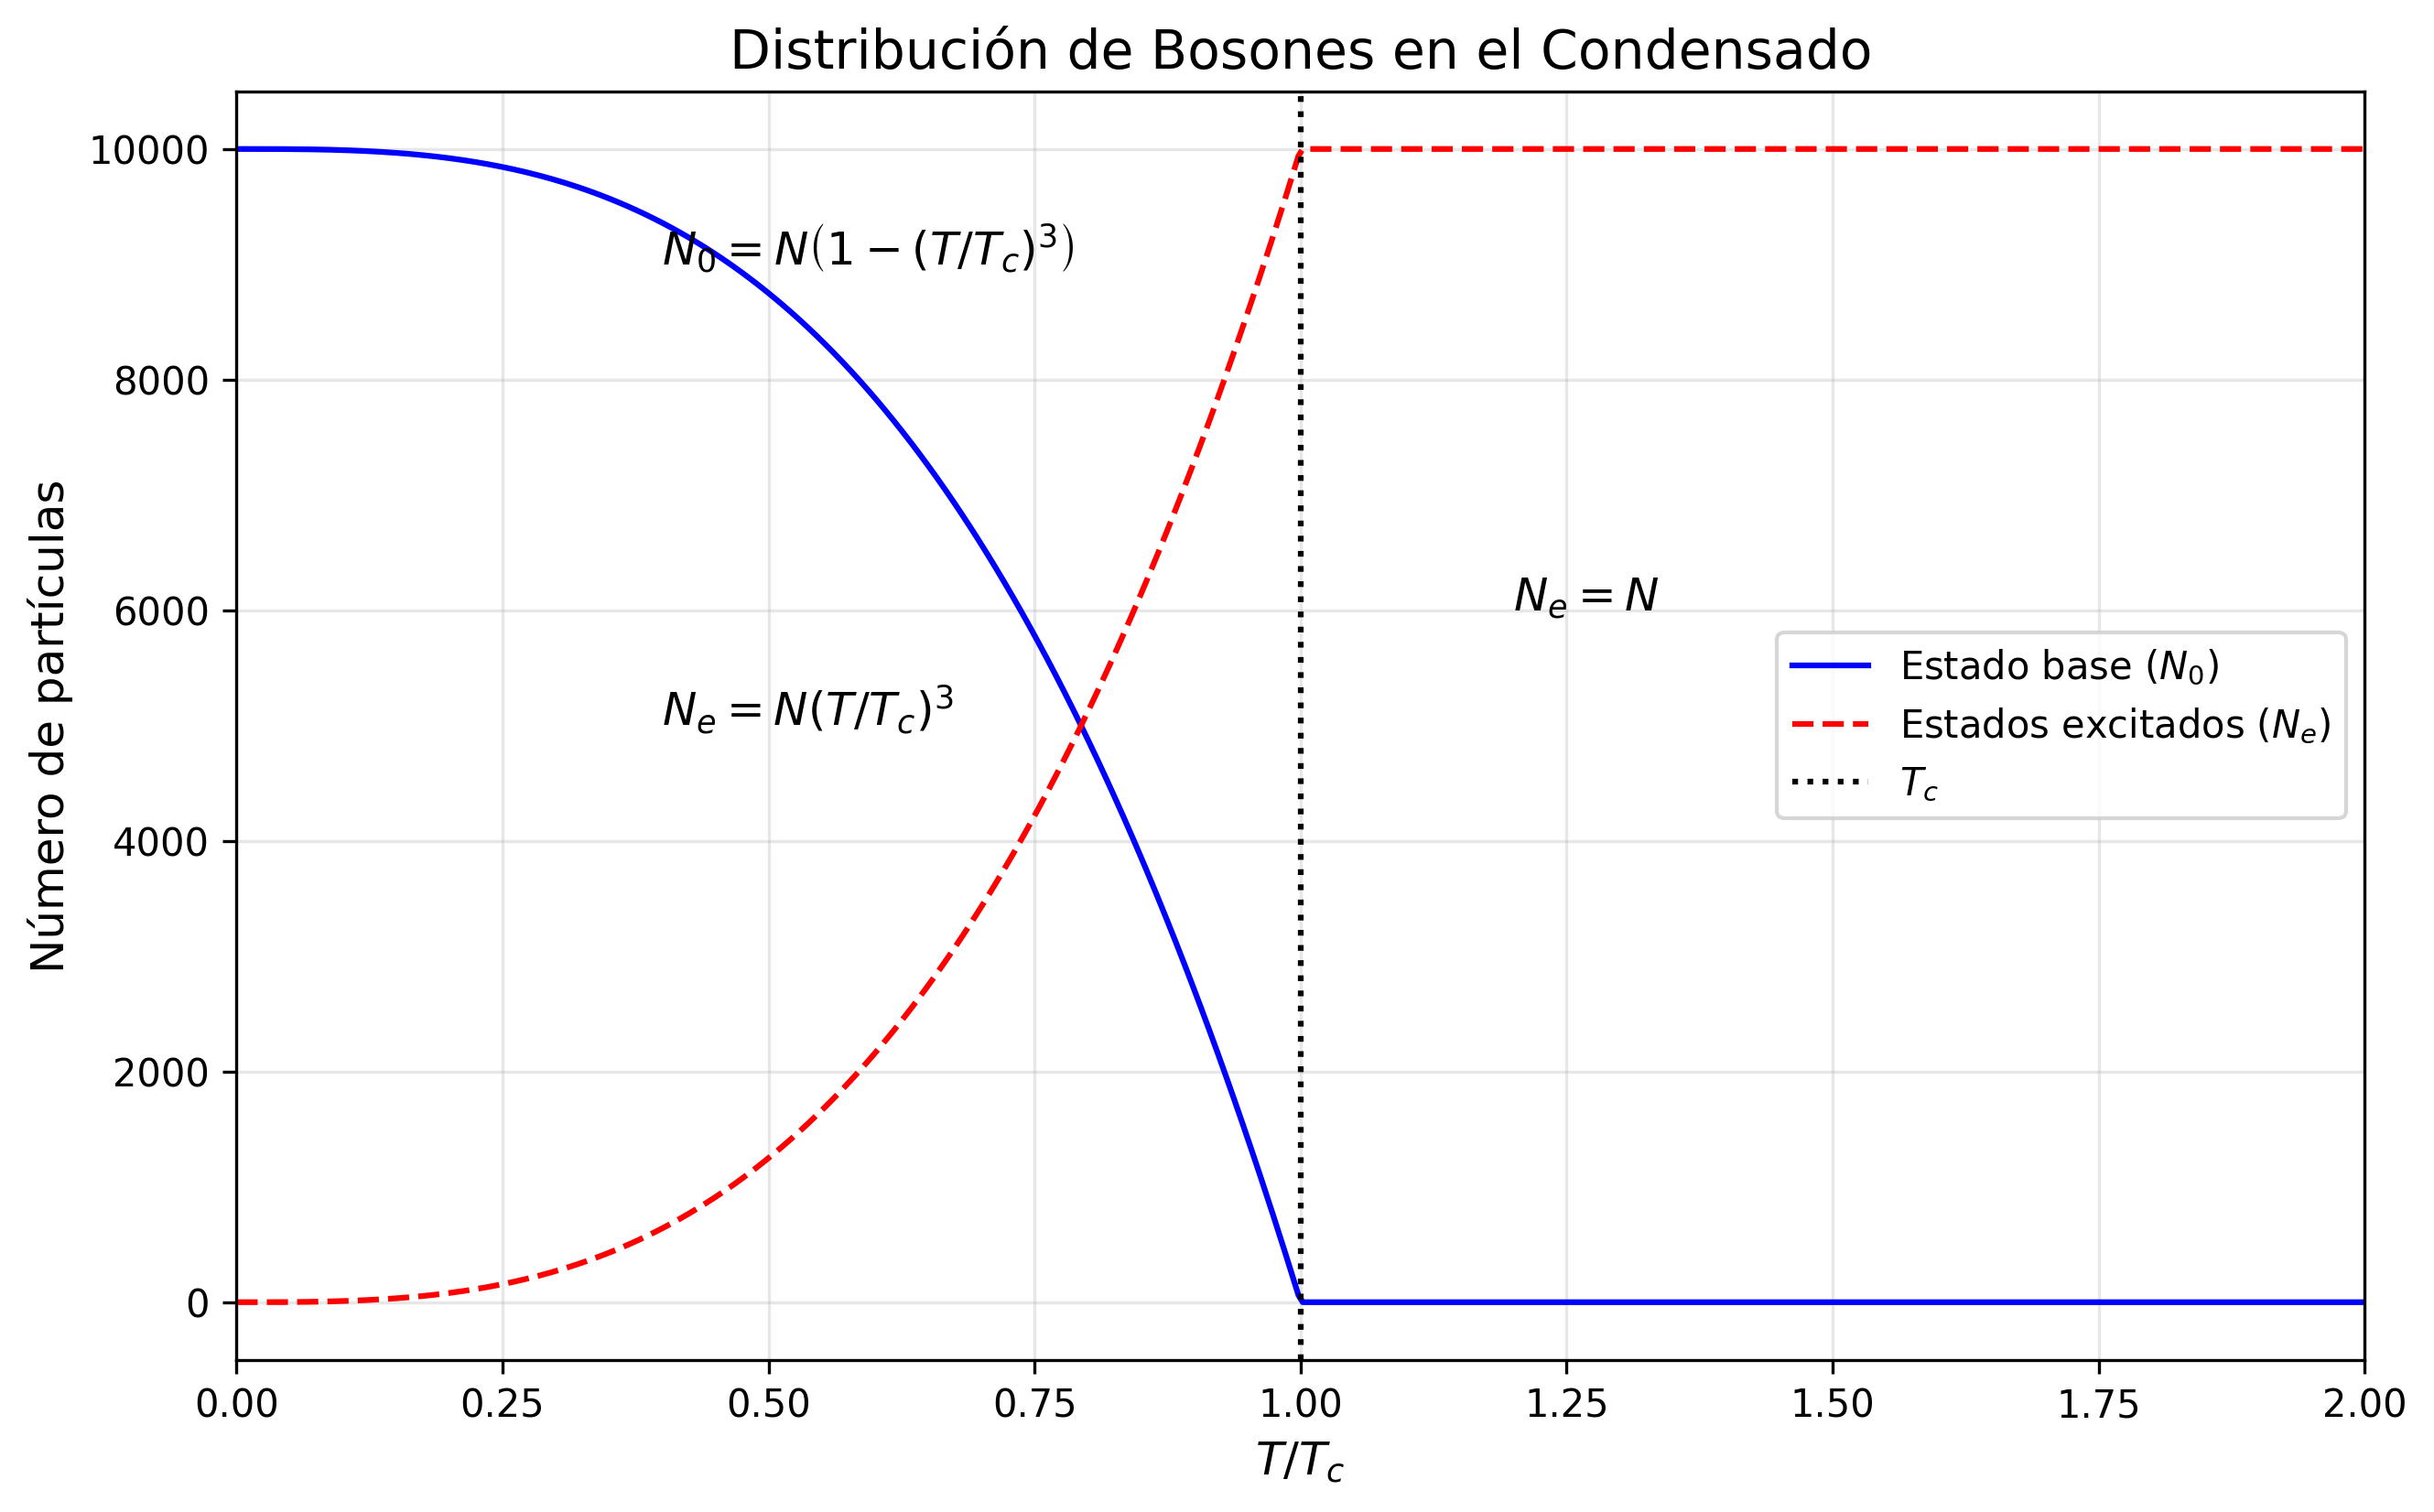
\includegraphics[width=0.85\textwidth]{code/n_0_N.png}
    \caption{Distribución de bosones en el estado base ($N_0$) y estados excitados ($N_e$) en función de $T/T_c$.}
    \label{fig:distribucion}
\end{figure}


Que fue obtenido con el codigo
\lstinputlisting{code/punto_3_f.py}

\section{G}

\section{H}

\subsection{$T \le T_c$}
Para hacer esto podemos partir desde:
\[
  U = \int_0^\infty \varepsilon g(\varepsilon) \frac{1}{e^{\frac{\varepsilon}{kT}} - 1} d\varepsilon
\]

Dado el $g(\varepsilon)$ ya encontrado podemos poner:
\begin{align*}
  U &= \int_0^\infty \varepsilon g(\varepsilon) \frac{1}{e^{\frac{\varepsilon}{kT}} - 1} d\varepsilon\\
  &= \int_0^\infty \frac{\varepsilon^3}{2 (\hbar \omega_0)^3} \frac{1}{e^{\frac{\varepsilon}{kT}} - 1} d\varepsilon\\
  &= \frac{1}{2 (\hbar \omega_0)^3}\int_0^\infty  \frac{\varepsilon^3}{e^{\frac{\varepsilon}{kT}} - 1} d\varepsilon\\
  x &= \frac{\varepsilon}{kT}\\
  \varepsilon &= x kT\\
  d\varepsilon &= kT dx\\
  U &= \frac{1}{2 (\hbar \omega_0)^3} \int_0^\infty  \frac{(x kT)^3}{e^{x} - 1} kT dx\\
  U &= \frac{1}{2 (\hbar \omega_0)^3} \int_0^\infty  (kT)^4 \frac{x^3}{e^{x} - 1} dx\\
  U &= \frac{(kT)^4}{2 (\hbar \omega_0)^3} \int_0^\infty   \frac{x^3}{e^{x} - 1} dx\\
\end{align*}

Ahora, el resultado de la integral 

\begin{align*}
  \int_0^\infty \frac{x^3}{e^x - 1} dx &= \Gamma(4)\zeta(3)\\
  &= 6 \zeta(3)
\end{align*}

Ahora teniendo
\[
  T_c = \frac{\hbar \omega_0}{k} \left( \frac{N}{\zeta(3)} \right)^{\frac{1}{3}}
\]

Con lo cual podemos reorganizarnos

\begin{align*}
  T_c &= \frac{\hbar \omega_0}{k} \left( \frac{N}{\zeta(3)} \right)^{1/3}\\
   \hbar \omega_0 &= k T_c \left( \frac{N}{\zeta(3)} \right)^{-1/3}\\
   (\hbar \omega_0)^3 &= k^3 T_c^3 \left( \frac{N}{\zeta(3)} \right)^{-1}\\
   U &= \frac{3 (kT)^4 \zeta(4)}{(\hbar \omega_0)^3}\\
   U &= \frac{3 (kT)^4 \zeta(4)}{k^3 T_c^3 \left( \frac{N}{\zeta(3)} \right)^{-1}} = \frac{3 (kT)^4 \zeta(4) N}{k^3 T_c^3 \zeta(3)}\\
   U &= \frac{3 k T^4 \zeta(4) N}{k^3 T_c^3 \zeta(3)} = \frac{3 T^4 N \zeta(4)}{k^2 T_c^3 \zeta(3)}\\
   U &= \frac{3 T^4 \zeta(4)}{k^2 T_c^3 \zeta(3)} \cdot \zeta(3) \left( \frac{k T_c}{\hbar \omega_0} \right)^3\\
   U &= 3 \left( \frac{T}{T_c} \right)^4 \frac{\zeta(4)}{\zeta(3)}\\
  U(T \leq T_c) &= 3 \left( \frac{T}{T_c} \right)^4 \frac{\zeta(4)}{\zeta(3)}\\
\end{align*}

\subsection{$T \ge T_c$}

En este caso la diferencia mas relevante es que:
\[
  U = \int_0^\infty \varepsilon g(\varepsilon) \frac{1}{z^{-1}e^{\frac{\varepsilon}{kT}} - 1} d\varepsilon
\]

Lo cual nos permite hacer exactamente el mismo desarrollo que antes cambiando la integral donde:

\begin{align*}
  \int_0^\infty \frac{x^3}{z^{-1} e^x - 1} dx &= \Gamma(4)g_4(z)\\
  &= 6 g_4 (z)
\end{align*}

Con esto entonces: 
\begin{align*}
  U &= \frac{6 (kT)^4}{2(\hbar \omega_0)^3} g_4(z) = \frac{3 (kT)^4}{(\hbar \omega_0)^3} g_4(z)\\
   (\hbar \omega_0)^3 &= \frac{k^3 T_c^3 \zeta(3)}{N}\\
   U &= \frac{3 (kT)^4}{\frac{k^3 T_c^3 \zeta(3)}{N}} g_4(z) = 3 \left( \frac{T}{T_c} \right)^4 \frac{g_4(z)}{\zeta(3)}\\
   U(T \geq T_c) &= 3 \left( \frac{T}{T_c} \right)^4 \frac{g_4(z)}{\zeta(3)}\\
\end{align*}

\section{I}

\subsection{$T < T_c$}

En este caso tenemos

\[
  U(T) = 3 \left( \frac{T}{T_c} \right)^4 \frac{\zeta(4)}{\zeta(3)} NkT_c
\]

Con esto entonces:
\begin{align*}
  C_V &= \frac{\partial U}{\partial T}\\
  &= 12\frac{\zeta(4)}{\zeta(3)}Nk\left(\frac{T}{T_c}\right)^3
\end{align*}

\subsection{$T < T_c$}

La energía incluye la fugacidad \( z \):  
\[
U(T \geq T_c) = 3 \left( \frac{T}{T_c} \right)^4 \frac{g_4(z)}{\zeta(3)} N k T_c.
\]  

Con esto entonces queda:

\[
  C_V = \frac{\partial U}{\partial T} = 12 \frac{g_4(z)}{\zeta(3)} N k \left( \frac{T}{T_c} \right)^3 - 9 \frac{g_3(z)^2}{\zeta(3) g_2(z)} N k \left( \frac{T}{T_c} \right)^3 \frac{dz}{dT}
\]


\subsection{$T_c$}

Límite \( T \to T_c^- \)
  \[
  C_V(T_c^-) = 12 \frac{\zeta(4)}{\zeta(3)} N k.
  \]  
Límite \( T \to T_c^+ \)
  \[
  C_V(T_c^+) = 12 \frac{\zeta(4)}{\zeta(3)} N k - 9 \frac{\zeta(3)}{\zeta(2)} N k.
  \]  
Discontinuidad:
  \[
  \Delta C_V = C_V(T_c^+) - C_V(T_c^-) = -9 \frac{\zeta(3)}{\zeta(2)} N k \approx -6.577 N k.
  \]

\subsection{Grafico}

Este grafico lo podemos hacer con codigo como sigue:
\lstinputlisting{code/punto_3_i.py}

Con lo cual producimos esta grafica:

\begin{figure}[H]
    \centering
    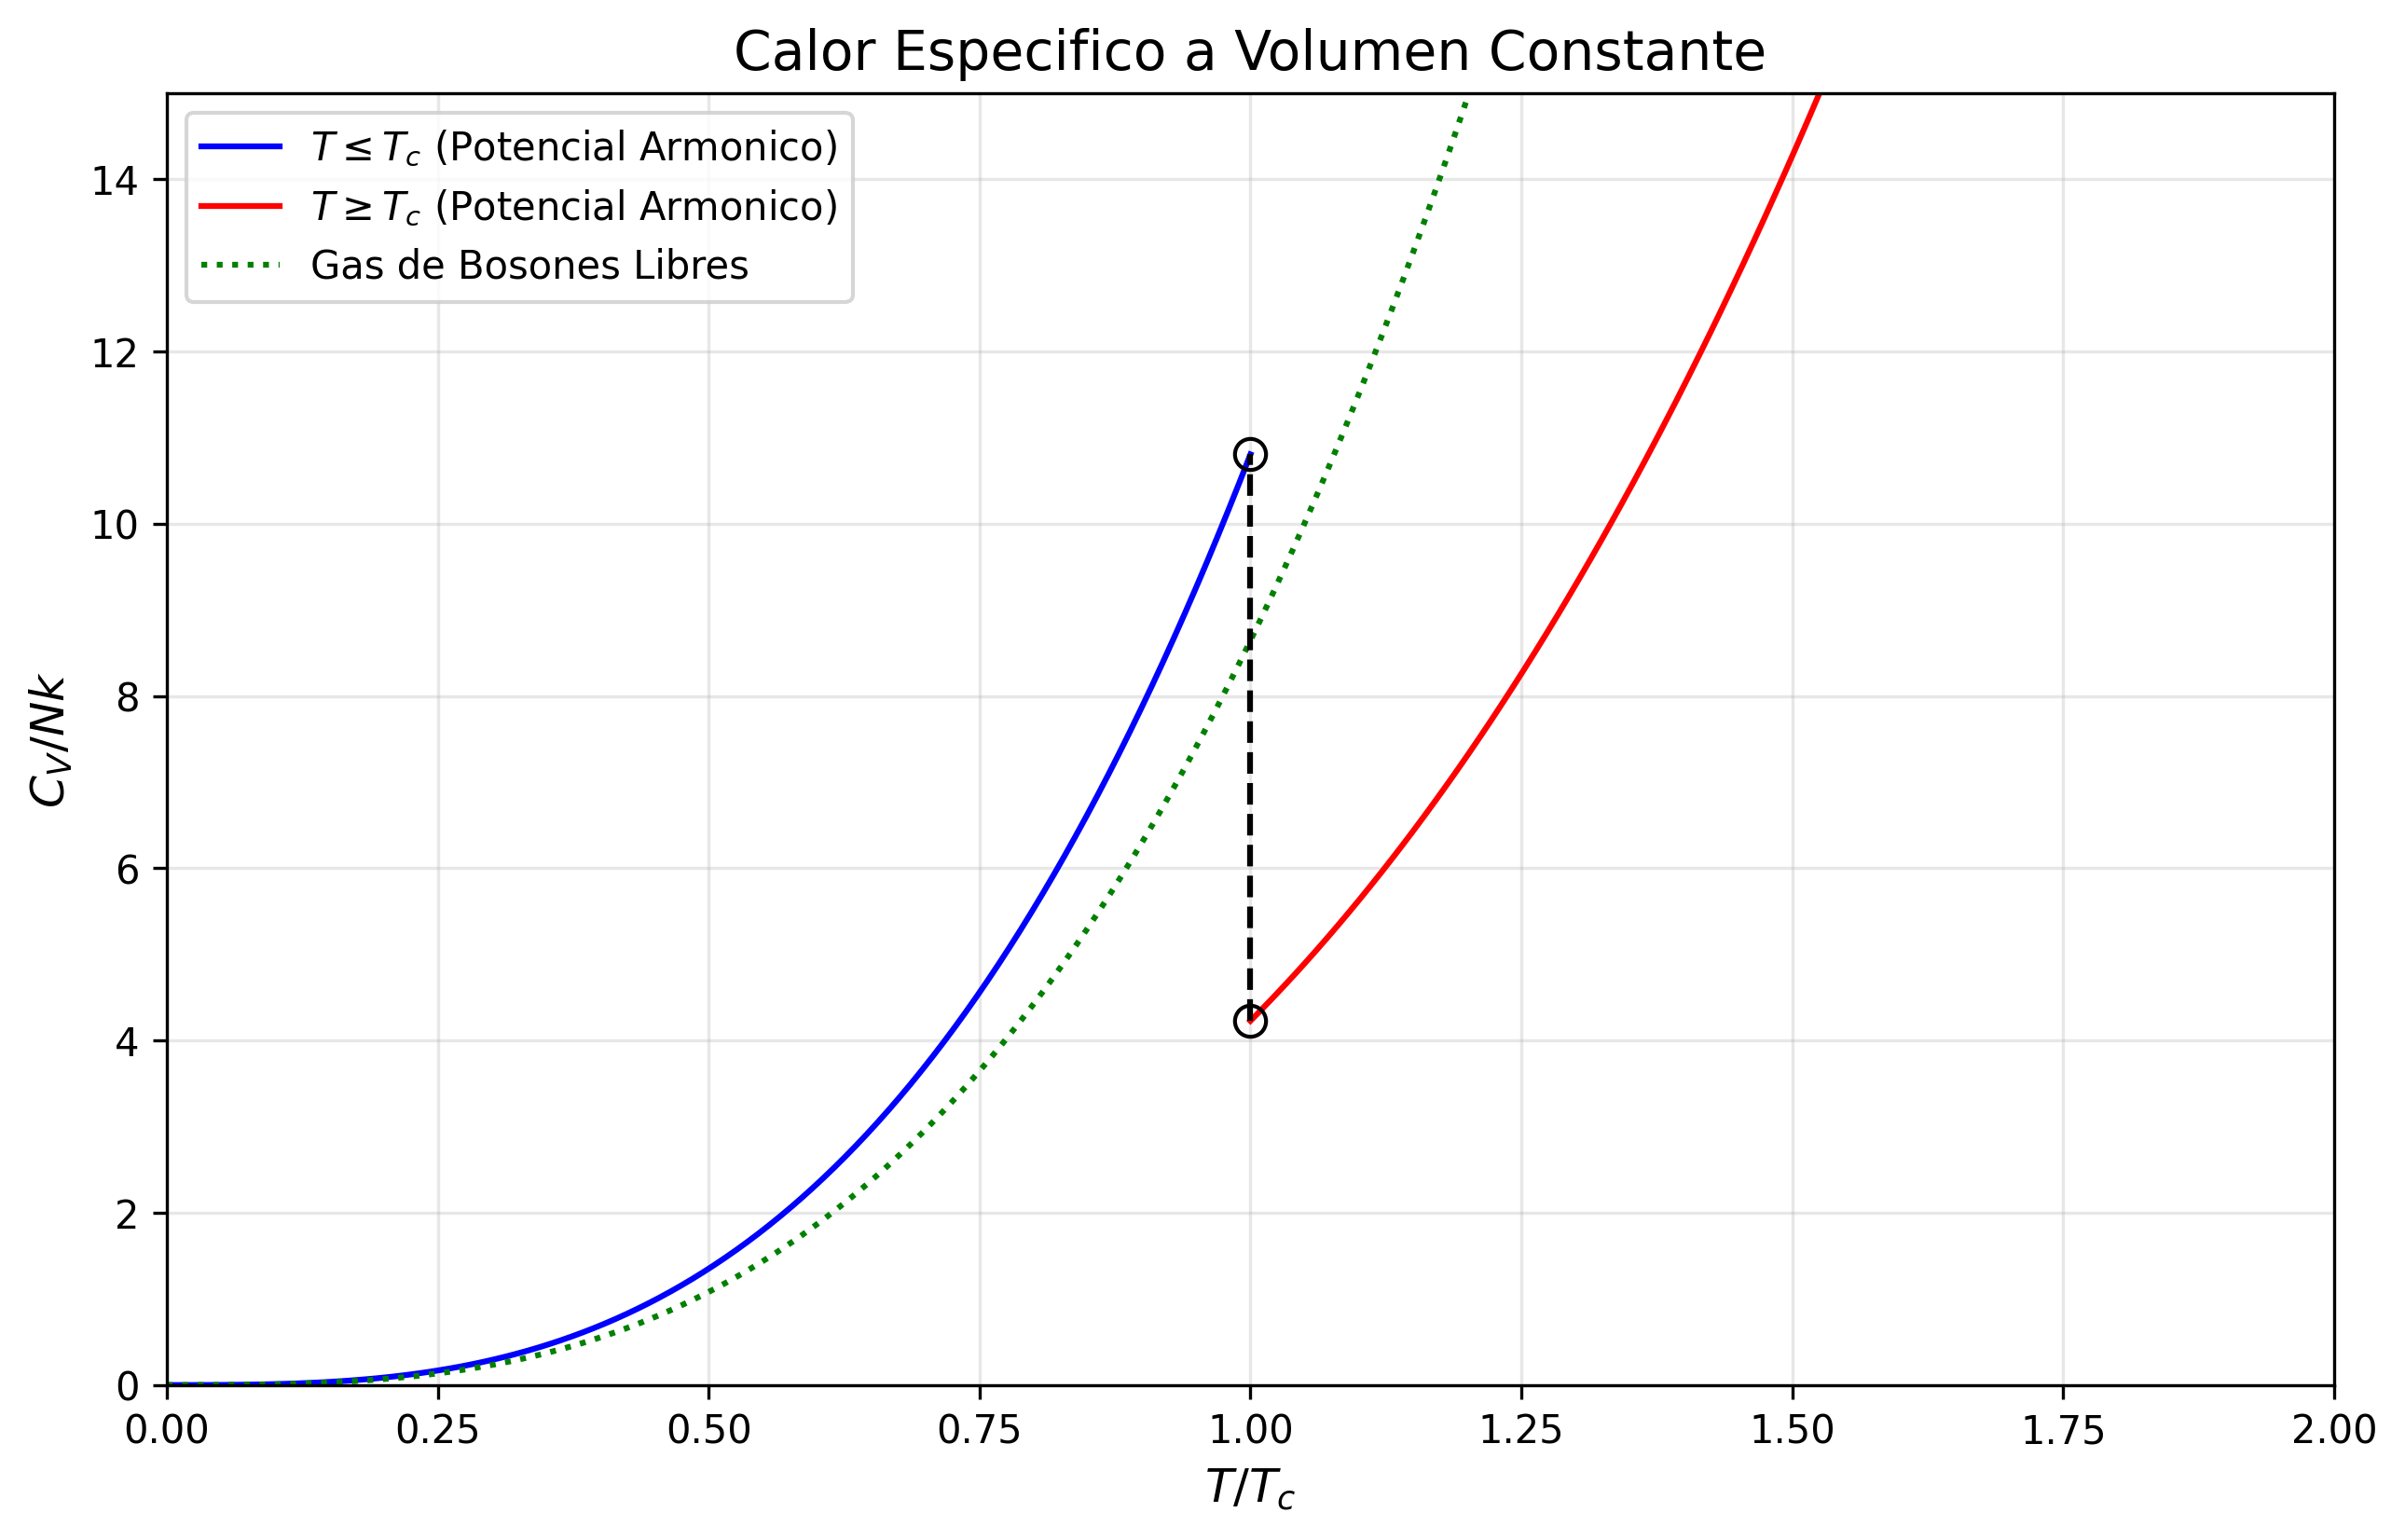
\includegraphics[width=0.9\textwidth]{./code/calor_especifico.png}
    \caption{Calor específico a volumen constante para el sistema en un potencial armónico y comparación con gas libre.}
    \label{fig:cv}
\end{figure}

\section{J}

\subsection{i}

\begin{enumerate}
   \item \( \omega_0 = 2\pi \times 100 \, \text{Hz} = 200\pi \, \text{rad/s} \).  
   \item \( \hbar = 1.054 \times 10^{-34} \, \text{J·s} \), \( k_B = 1.38 \times 10^{-23} \, \text{J/K} \).  
   \item \( N = 2 \times 10^4 \), \( \zeta(3) \approx 1.202 \).  
\end{enumerate}

Reemplazando queda

   \[
   T_c = \frac{(1.054 \times 10^{-34})(200\pi)}{1.38 \times 10^{-23}} \left( \frac{2 \times 10^4}{1.202} \right)^{1/3} \approx 122 \, \text{nK}.
   \]

Ahora para $\lambda$ a $T_c$
   Para \( ^{87}\text{Rb} \) (\( m \approx 1.44 \times 10^{-25} \, \text{kg} \)):  

   \[
   \lambda = \sqrt{\frac{2\pi \hbar^2}{m k_B T_c}} \approx 0.54 \, \mu\text{m}.
   \]

   Para la discontinuidad queda como:
   \[
   \Delta C_V \approx -6.577 N k_B = -6.577 \times (2 \times 10^4) \times 1.38 \times 10^{-23} \approx -1.82 \times 10^{-18} \, \text{J/K}.
   \]

\subsection{ii}
\subsubsection{$^{87}\text{Rb}$}
Usando el articulo Observation of Bose-Einstein Condensation in a Dilute Atomic Vapor disponible en Science en \url{https://www.science.org/doi/10.1126/science.269.5221.198}
  \begin{enumerate}
  \item \( T_c \approx 170 \, \text{nK} \).
  \item \( \lambda \approx 1 \, \mu\text{m} \).  
  \end{enumerate}

\subsubsection{$^{23}\text{Na}$}

Basandonos en el articulo Bose-Einstein Condensation in a Gas of Sodium Atoms \url{https://journals.aps.org/prl/abstract/10.1103/PhysRevLett.75.3969}

  \begin{enumerate}
  \item \( T_c \approx 500 \, \text{nK} \) (experimentos de Ketterle, 1995).  
  \end{enumerate}

Con lo cual nuestros resultados parecen estar apuntando en la dirección correcta.

\subsection{iii}


\end{document}
